\documentclass[a4paper, 10pt]{report}

\usepackage[right=1in, left=1in, top=1in, bottom=1in]{geometry}
\linespread{1.5}
\usepackage{amsmath, amsthm, amssymb} %math's packages
\usepackage[utf8]{inputenc} %document encoding

\usepackage{amsmath, amsthm, amssymb}
\usepackage{enumerate}
\usepackage{verbatim}
%\usepackage{indentfirst}
\usepackage{graphicx}
\usepackage{algorithm}
\usepackage{algpseudocode}
\usepackage{listings}
\usepackage{color}
\usepackage{subcaption}
\usepackage{hyperref}
\usepackage{float}
\usepackage[T1]{fontenc}
\usepackage{makecell}
\usepackage{colortbl}
\usepackage{booktabs}
%\usepackage{babel}
\usepackage{array,multirow,graphicx}
\usepackage{pgfplots} %plots
\usepackage{standalone} %including other files without preambule
\usepackage{setspace}
\usepackage{tabu}
\usepackage{pdfpages}


\newcommand{\cov}{\mathbb{C}\text{ov}}
\newcommand{\eig}{\text{EIG}}
\newcommand{\ape}{\text{APE}}
\newcommand{\kl}[2]{\text{KL}\left(\ #1\ ||\ #2\ \right)}
\newcommand{\entropy}[1]{H\left(\ #1\ \right)}
\newcommand{\expect}{\mathbb{E}}
\newcommand{\argmax}{\text{argmax}}
\newcommand{\simiid}{\overset{\text{\tiny iid}}{\sim}}
\newcommand{\qp}{q_p}
\newcommand{\qm}{q_m}
\newcommand{\ql}{q_\ell}
\newcommand{\R}{\mathbb{R}}
\newcommand{\prob}{\mathbb{P}}	
\newcommand{\tP}{\tilde{P}}	
\newcommand{\tPg}{\tilde{P}_{\gamma}}	
\newcommand{\tpi}{\tilde{\pi}}	
\newcommand{\tpig}{\tilde{\pi}_{\gamma}}
\newcommand{\tpigLi}{\tilde{P}_{\gamma,L,i}} 
\newcommand{\tpigLk}{\tilde{P}_{\gamma,L,k}} 
\newcommand{\tpigJi}{\tilde{P}_{\gamma,J,i}} 
\newcommand{\tpigJk}{\tilde{P}_{\gamma,J,k}} 
\newcommand{\RJi}{R_{\gamma,J,i}} 
\newcommand{\RJk}{R_{\gamma,J,k}}
\newcommand{\RLi}{R_{\gamma,L,i}} 
\newcommand{\RLk}{R_{\gamma,L,k}}
\newcommand{\Qgi}{Q_{\gamma,i}} 
\newcommand{\Qgk}{Q_{\gamma,k}}
\newcommand{\E}{\mathbb{E}}
\newcommand{\x}{\mathbf{x}}
\newcommand{\y}{\mathbf{y}}
\newcommand{\z}{\mathbf{z}}
\newcommand{\bu}{\mathbf{u}}
\newcommand{\bv}{\mathbf{v}}
\newcommand{\w}{\mathbf{w}}
\newcommand{\iid}{\overset{\scriptstyle{\text{i.i.d.}}}{\sim}}

\newcommand{\agi}{a_{\gamma,i}} 
\newcommand{\agk}{a_{\gamma,k}}  
\newcommand{\agj}{a_{\gamma,j}}  
\newcommand{\wgi}{w_{\gamma,i}} 
\newcommand{\wgk}{w_{\gamma,k}}
\newcommand{\wgj}{w_{\gamma,j}}
\newcommand{\giY}{\gamma \in \mathcal{Y}} 
\newcommand{\bb}[1]{\mathbb{#1}}
\theoremstyle{plain}
\newtheorem{thm}{Theorem}%[section]
\newtheorem{assu}[thm]{Assumption}
\newtheorem{prop}[thm]{Proposition}
\newtheorem{lemma}[thm]{Lemma}
\newtheorem{cor}[thm]{Corollary}
%
\theoremstyle{definition}
\newtheorem{ex}[thm]{Example}
\newtheorem{defi}[thm]{Definition}
\newtheorem{alg}{Algorithm}
%
\theoremstyle{remark}
\newtheorem{remark}[thm]{Remark}
\renewcommand{\baselinestretch}{1.5}

\begin{document}
	
	\documentclass[TRANSFER_THESIS.tex]{subfiles}
\begin{document}
\thispagestyle{empty}
\begin{titlepage}
\begin{center}
\hfill 
\includegraphics[width=2.0in]{figures/Dept_Stats_logo_vertical_CMYK.eps} \hfill \phantom{.} \\
\vspace{2.5cm}
\rule{\textwidth}{0.5mm} \\ [16pt]
\Huge {\bfseries Variational, Monte Carlo and Policy-Based Approaches to Bayesian Experimental Design}
\rule{\textwidth}{0.5mm} \\ [4pt]
\vfill
\Large {A thesis submitted for the degree of \\ \emph{Doctor of Philosophy}} \\
\vspace{1cm}
\large \textsc{Michaelmas 2021} \\
\rule{\textwidth}{0.5mm} \\ [4pt]
{\fontsize{14}{14}\textsc{Adam Evan Foster} \hfill \textsc{Department of Statistics}} \\ [8pt]
{\fontsize{14}{14} \textsc{University College \hfill University of Oxford}}
\rule{\textwidth}{0.5mm} \\ [4pt]
\end{center}
\vspace{2cm}
\end{titlepage}
\end{document}


	
	\newpage
	\chapter*{Abstract}
	Bayesian experimental design (BED) is a powerful mathematical framework with diverse applications that include asking the most pertinent question in an online survey, designing a laboratory experiment, choosing sensor locations, obtaining labels in active learning, searching for the maximum of an unknown function, and exploring an unknown environment.
	Automated design of optimal experiments allows scientists to undertake experiments more efficiently, reach statistically valid conclusions more quickly, and unlock kinds of experiments that have been hitherto considered impractical.
	Unfortunately, widespread utilisation of BED for designing optimal experiments is not yet a reality.
	Adoption of BED is hampered by computational challenges that are inherent in finding experimental designs that maximise the expected information that will be gained about the underlying process by running the experiment.
	Broadly, the computational challenges can be broken down into three parts of increasing complexity: 1) estimating the expected information gain, 2) optimising the expected information gain over the space of possible designs, and 3) choosing a sequence of optimal designs whilst incorporating feedback from the experiment.
	
	The goal of this thesis is to present methods to tackle these computational challenges by taking inspiration from the rapid development of modern probabilistic machine learning in areas such as variational inference, amortised inference, stochastic gradient optimisation, probabilistic deep learning, Monte Carlo methods, likelihood-free inference, constrastive learning and reinforcement learning.
	We show how concepts from these areas can be brought together to create a modern approach to BED that begins to overcome the computational restrictions on the Bayesian design of experiments.
	
	Specifically, we begin by presenting advances in the estimation of expected information gain, incorporating ideas from variational and amortised inference.
	We make several contributions to the optimisation of experimental designs using stochastic gradient methods.
	Finally, we turn to the sequential design problem, and demonstrate how efficient, adaptive design may be achieved through the use of a policy.
	In concert, these methods allow us to expand the range of circumstances in which BED can be used to design optimal experiments, with implications for both machine learning and the sciences.

	
	\newpage
	\chapter*{Acknowledgements}
	I would like to begin by thanking my supervisors Yee Whye Teh and Tom Rainforth for their kindness, patience and guidance throughout my DPhil.
	To Yee Whye, I particularly owe gratitude for his thoughtfulness and calmness, the confidence he has in me and his unwavering commitment to allow me to work on whichever project I find most interesting.
	To Tom, I would like to express my thanks for the enthusiasm and interest he has for our shared work---I would have given up many years ago without his input and his drive to continually improve our understanding---and for teaching me many of the skills that I needed to succeed in my DPhil, including writing in something other than the `Russian mathematician' style.
	
	In the Department of Statistics at Oxford, I would like to thank Emile Mathieu for his friendship and support during our four year DPhil adventure, as well as Benjamin Bloem-Reddy, Chris Maddison, Dominic Richards, Jean-François Ton, Adam Kosiorek, Emilien Dupont, Anthony Caterini, Adam Goliński, Bobby He, Hyunjik Kim, Qinyi Zhang, Yuan Zhou, Michael Hutchinson and Desi Ivanova for their friendship and for making the department a good place to be.
	
	I also owe a huge debt of gratitude to Noah Goodman for his inspiration and guidance during my time at Uber AI Labs, and for helping to set me on the exciting research path that this thesis is a partial culmination of.
	I would also like to thank Martin Jankowiak for his help and support with our joint research, as well as Eli Bingham, Paul Horsfall and the whole of the Pyro team for good times both in the office and out of it.
	To Takashi Goda, Tomohiko Hironaka and Wataru Kitade of the University of Tokyo I express my gratitude for their willingness to collaborate and share their expertise on MLMC.
	To Rattana Pukdee, Ilyas Malik and Matthew O'Meara, thank you for being wonderful co-authors.
	I am grateful to Árpi Vezér, Craig Glastonbury, Páidí Creed, Sam Abujudeh and Aaron Sim for their kindness and help during my time as an intern at BenevolentAI.
	This research would not have been possible without the generous financial suppport that I received from an EPSRC Excellence Award.
	
	Finally, I would like to thank the friends and family who have been with me during the highs and lows of my studies.
	I am humbled by the kindness that my parents, siblings, and family have always shown me.
	To Diallo, thank you for the love and support that has sustained me on the last leg of my DPhil journey.
	To my friends from University College---James, Seb, Miles, Tales, Nonie, Colm, Mitch \& Jess, Max and Rieke---thank you for so many happy memories of Oxford.
	And to Alexander Temple McCune for being the man you were and my friend, thank you.
	
	
	\tableofcontents
	
	\section*{Page counts}
	\begin{center}
		\begin{tabular}{lr}
			Main content pages & 100 \\
			Reference pages & 50 \\
			Appendices & 25 \\
			Other & \\
			\hline
			Total & 100
		\end{tabular}
	\end{center}
	
\newpage
	
	
	\chapter{Introduction and Literature Review}
	\label{chap:intro}
	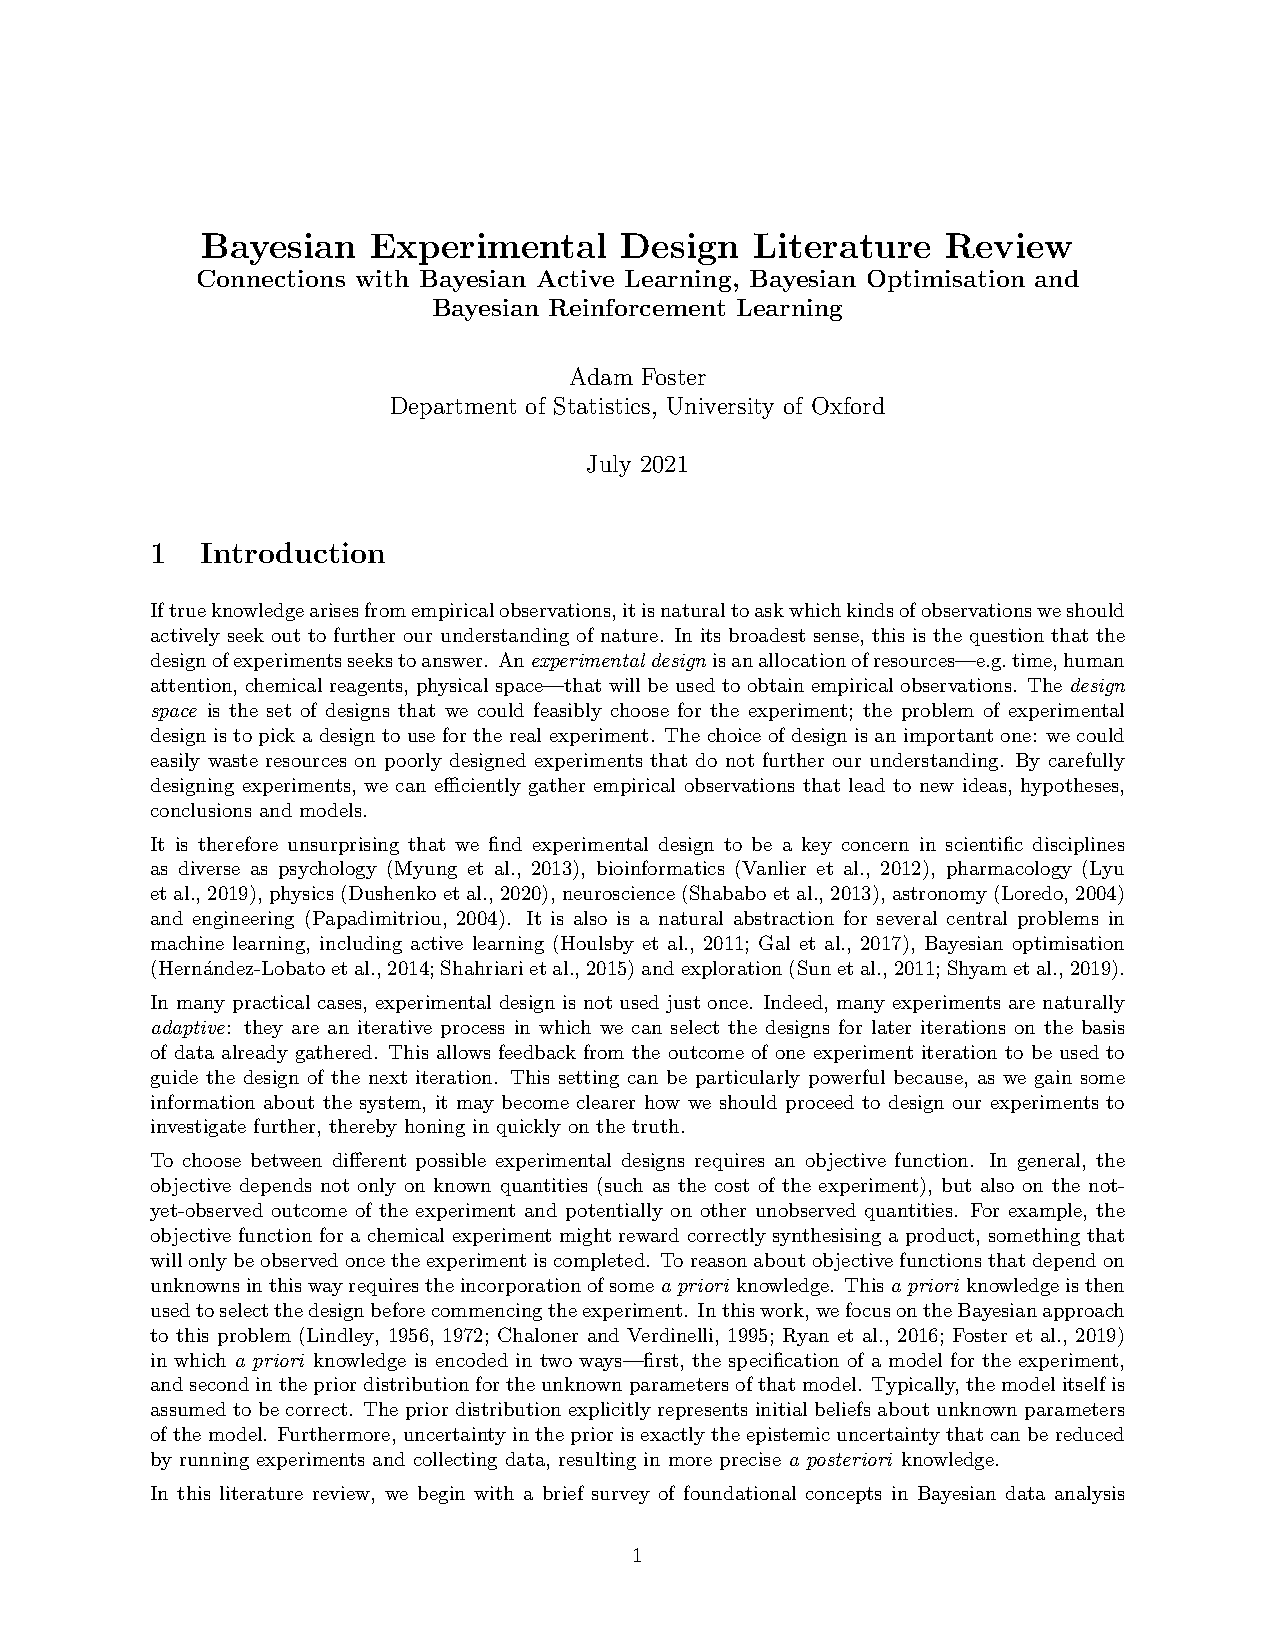
\includepdf[pagecommand={}, pages=-, trim=0mm 17.5mm 0mm 17.5mm, clip]{litreview.pdf}
	
	\chapter{Variational Bayesian Optimal Experimental Design}
	\label{chap:vboed}
	\includepdf[pagecommand={}, pages=-, trim=5mm 17.5mm 5mm 17.5mm, clip]{vboedmain.pdf}
	\includepdf[pagecommand={}, pages=-, trim=5mm 17.5mm 5mm 17.5mm, clip]{vboedsupplement.pdf}
	
	\chapter{A Unified Stochastic Gradient Approach to Designing Bayesian-Optimal Experiments}
	\label{chap:sgboed}
	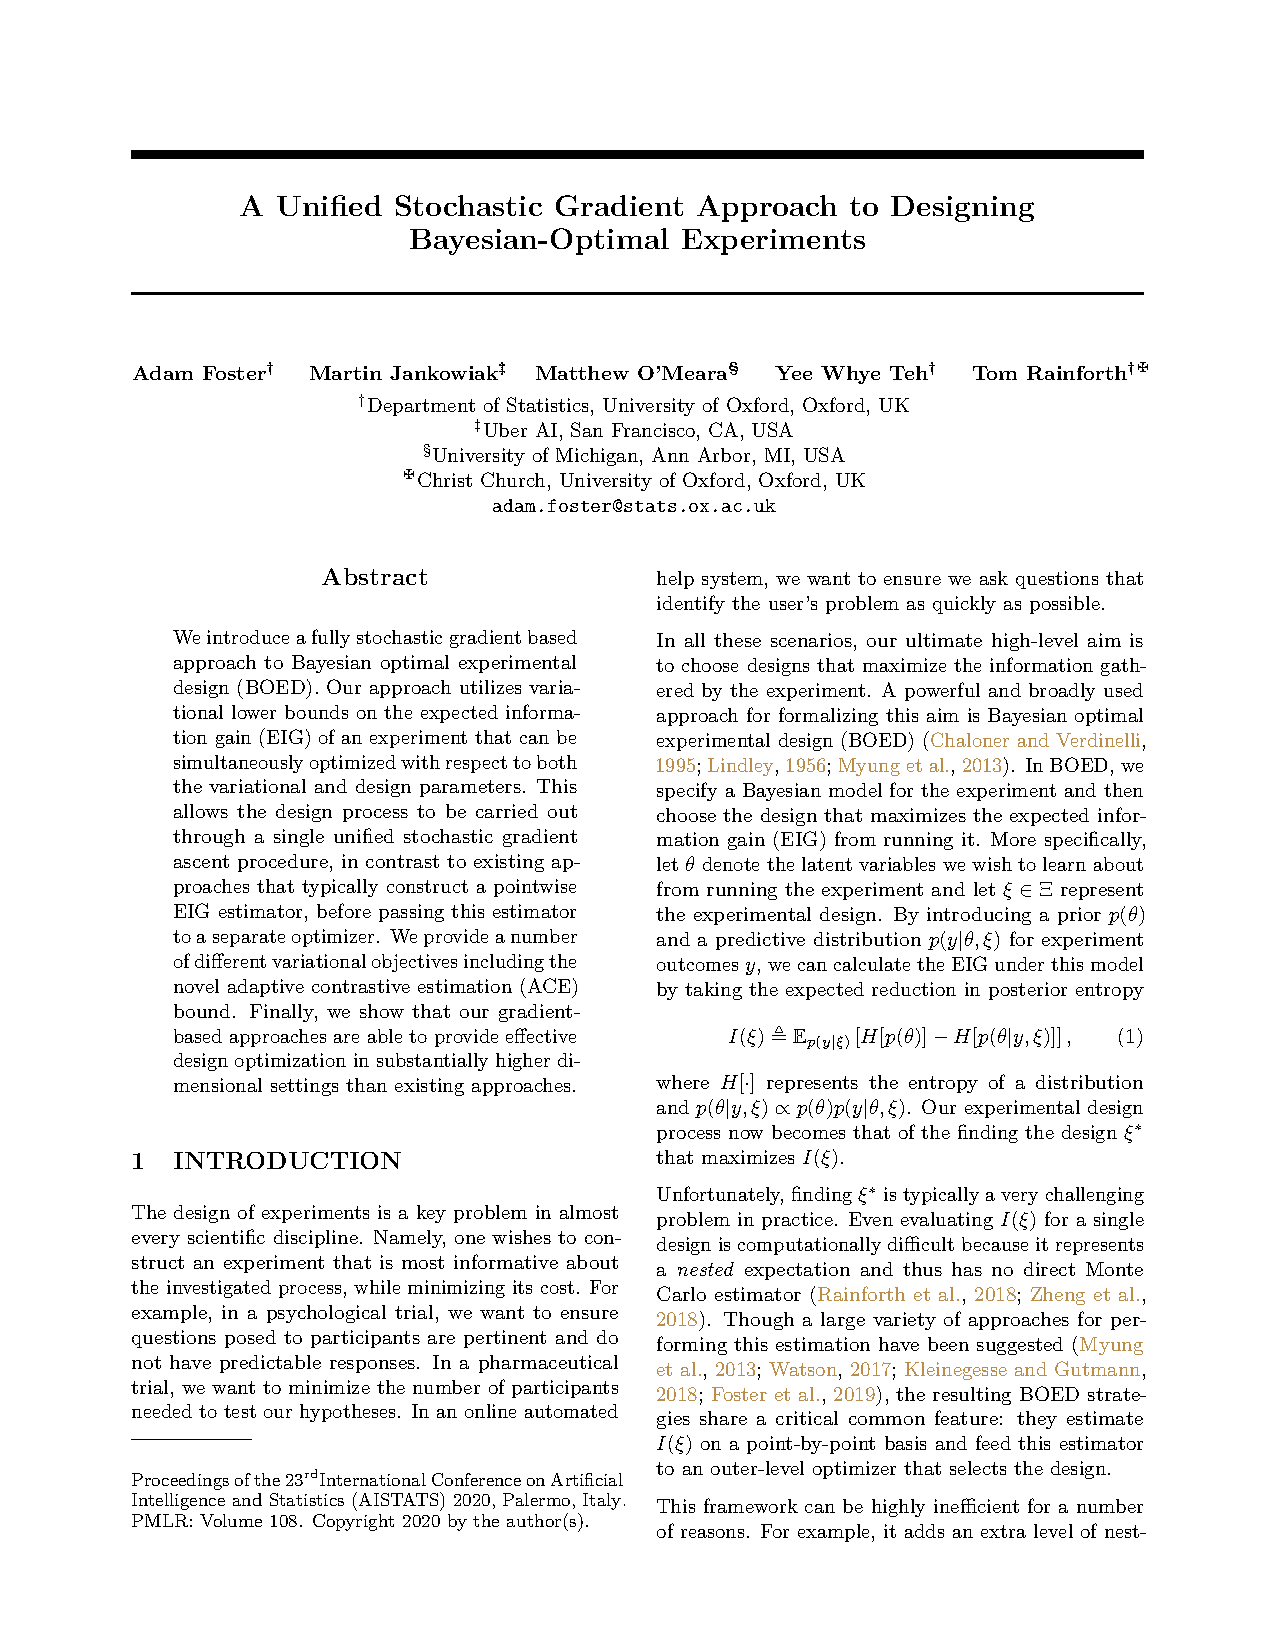
\includepdf[pagecommand={}, pages=-, trim=0mm 16.5mm 0mm 16.5mm, clip]{sgboed.pdf}
	
	\chapter{Unbiased MLMC stochastic gradient-based optimization of Bayesian experimental designs}
	\label{chap:mlmc}
	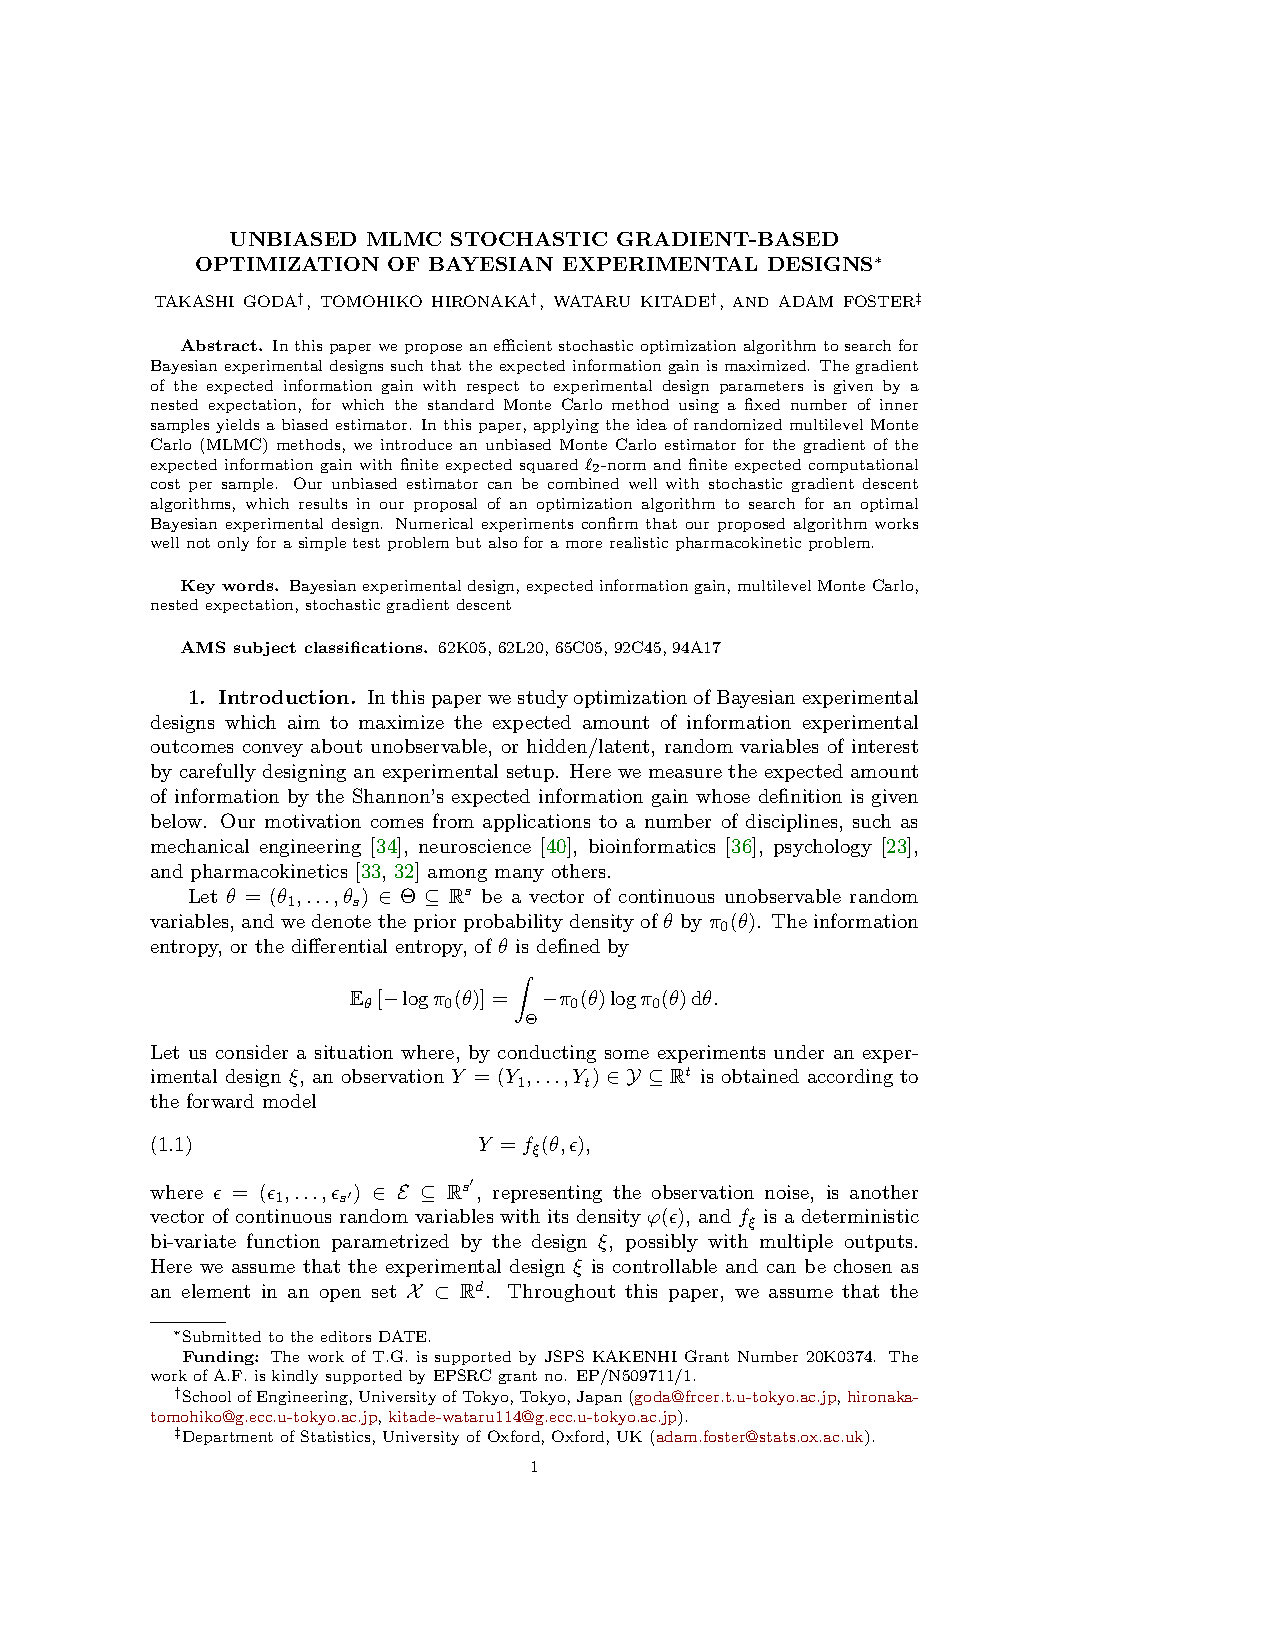
\includepdf[pagecommand={}, pages=-, trim=0mm 33mm 32mm 30mm, clip]{mlmc.pdf}
	
	\chapter{Deep Adaptive Design: Amortizing Bayesian Experimental Design}
	\label{chap:dad}
	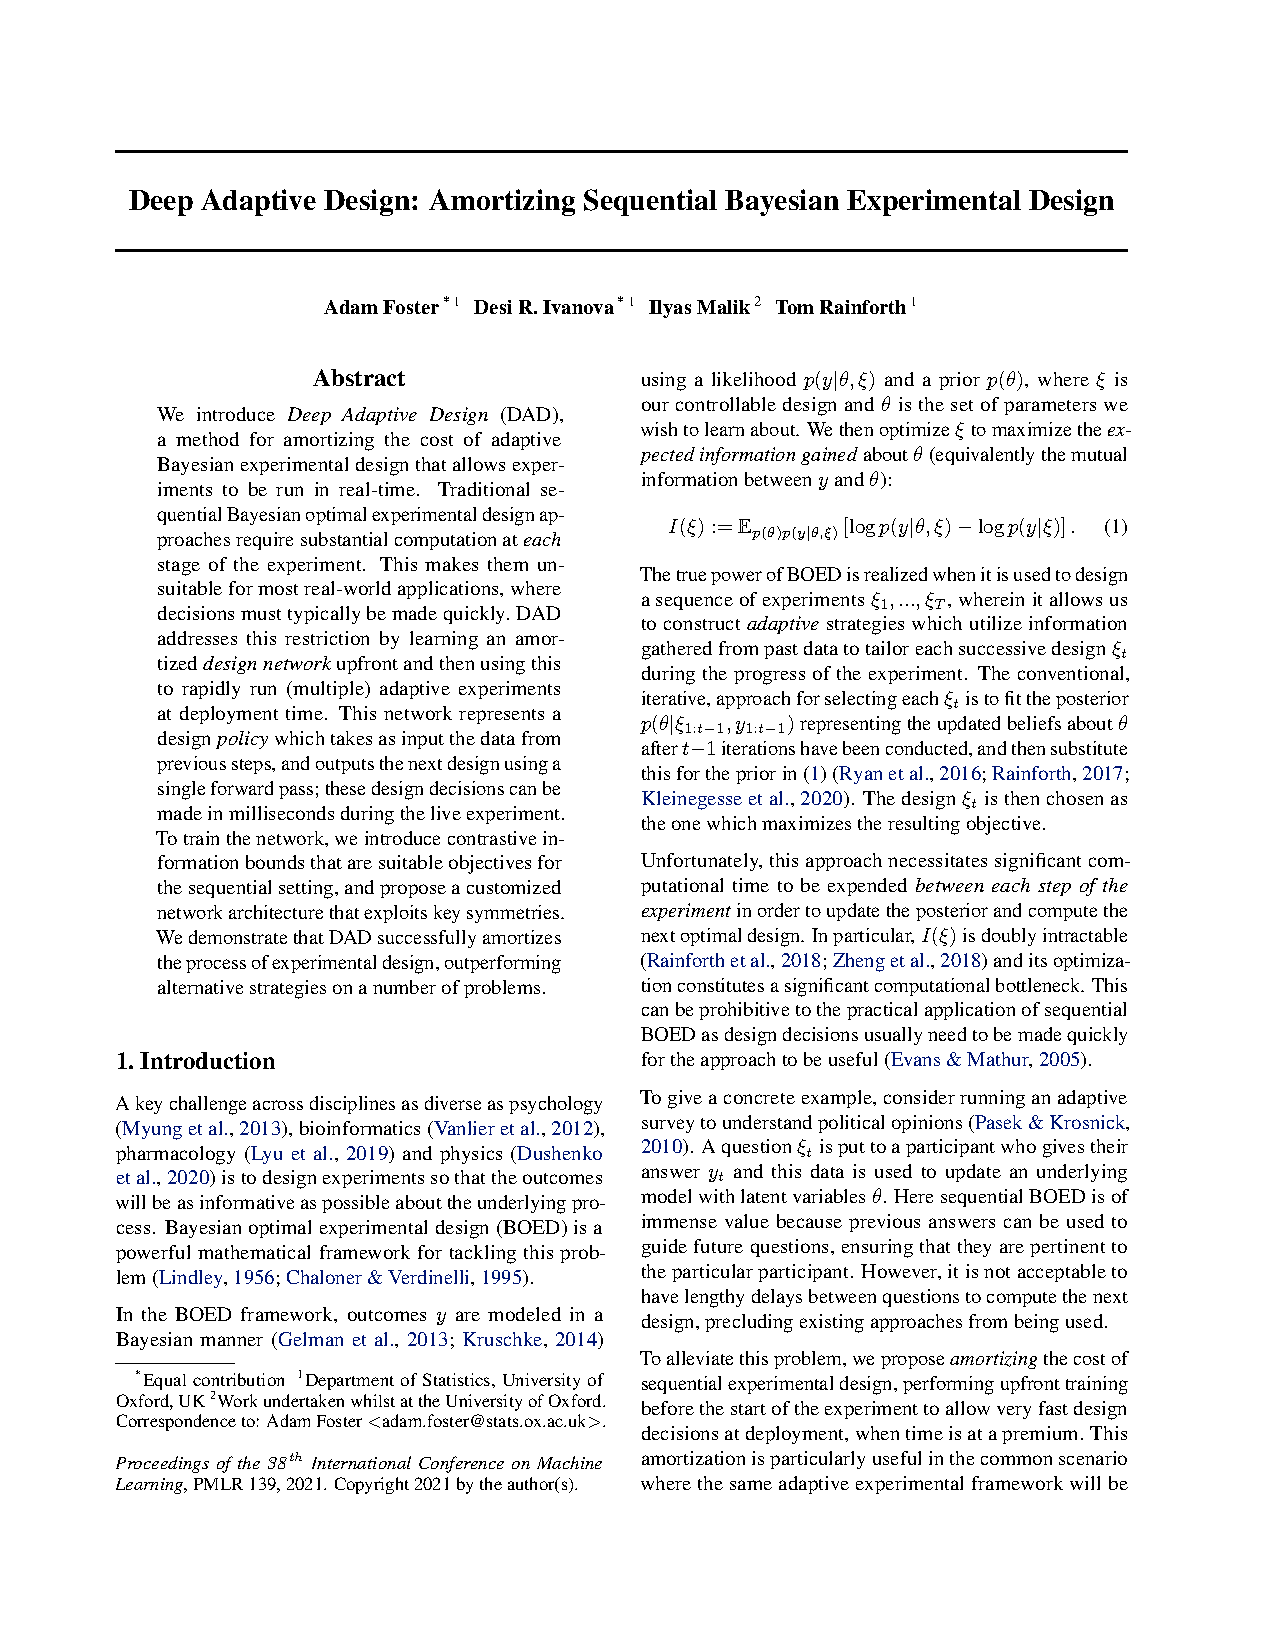
\includepdf[pagecommand={}, pages=-, trim=0mm 17mm 0mm 17mm, clip]{dad.pdf}
	
	\chapter{Implicit Deep Adaptive Design: Policy-Based Experimental Design without Likelihoods}
	\label{chap:idad}
	
	\chapter{Additional material}
	\label{chap:additional}
	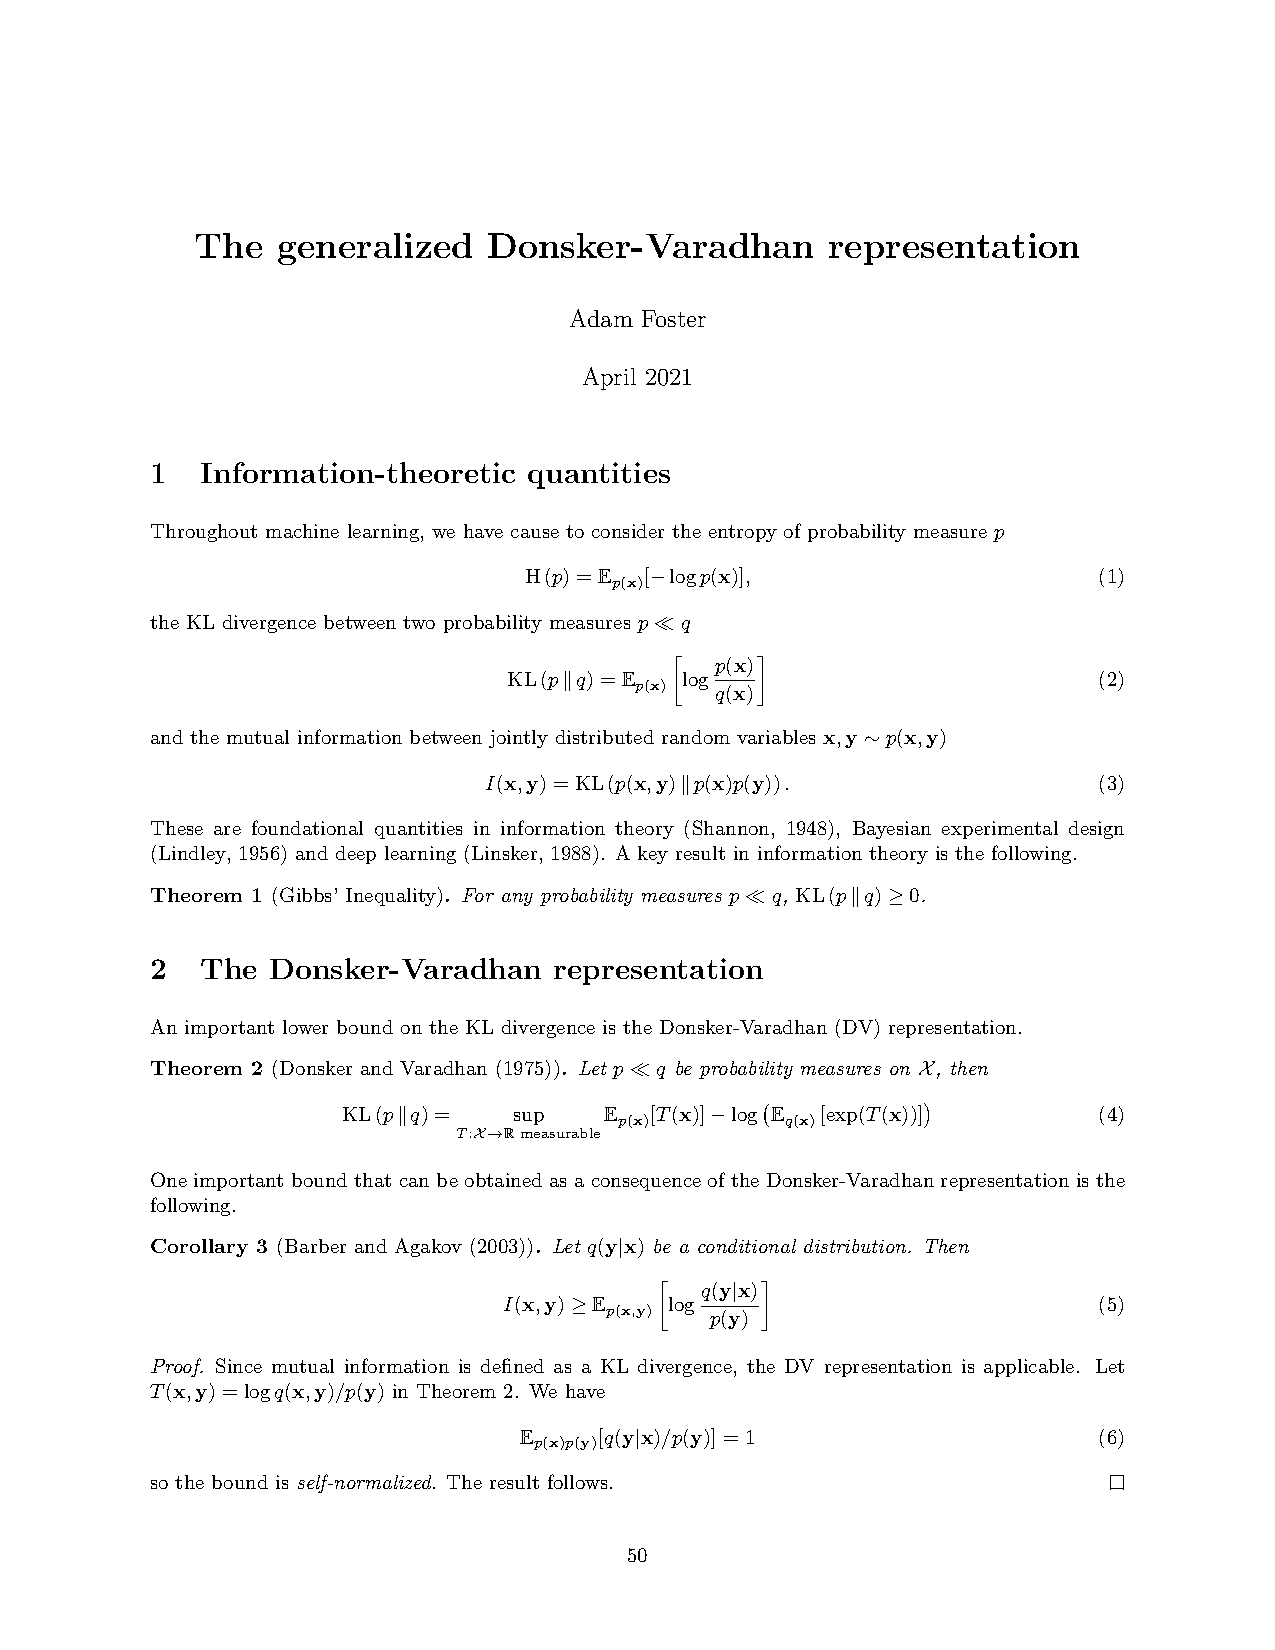
\includepdf[pages=-]{bounds.pdf}
	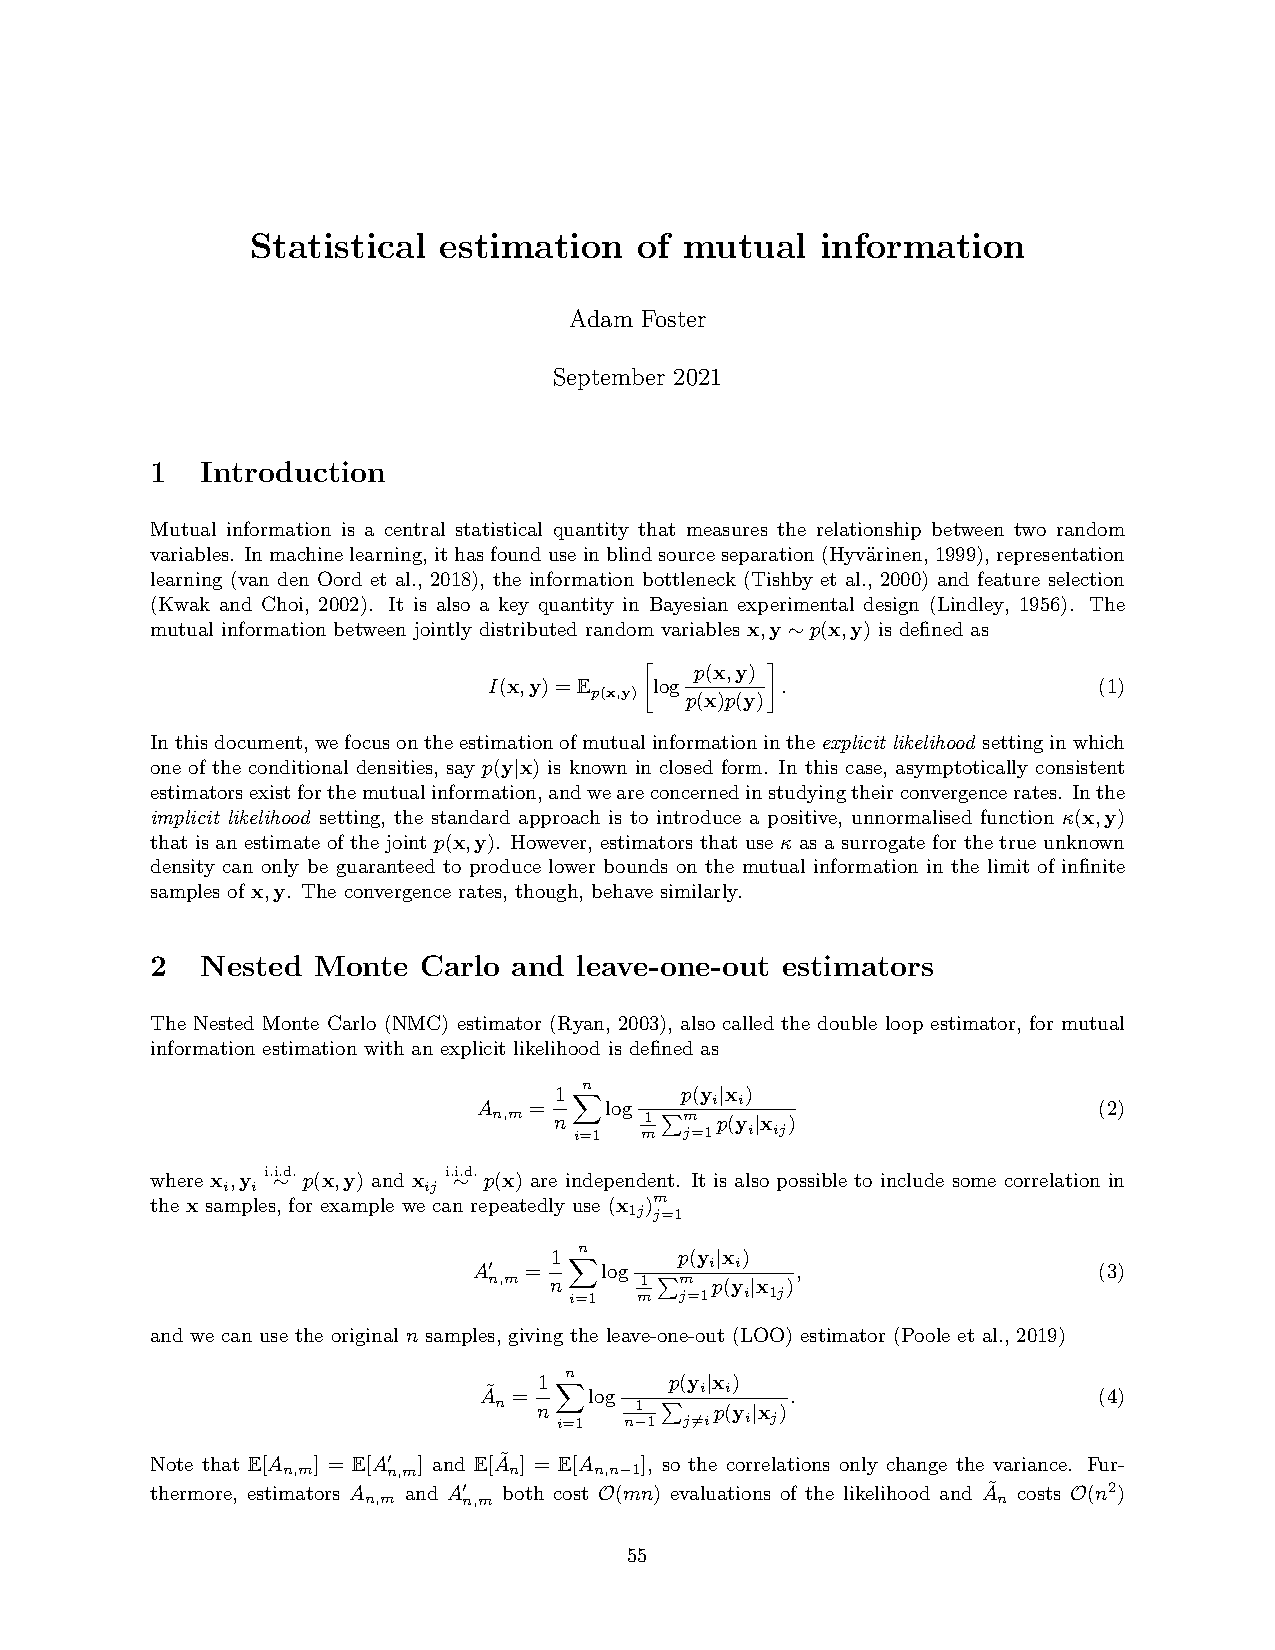
\includepdf[pages=-]{estimator.pdf}
	
	\chapter{Discussion}
	\label{chap:discussion}
	
	
	
\end{document}